\section{Introduction}
\label{sec:introduction}
% task introduction
The popular smartphones with high quality cameras have enabled people to capture events all over the world by videos and share them via social media conveniently.  
When an event happens, different cameras may record it at different positions from different perspectives of view.
For example, videos from surveillance cameras usually record the event from a fixed location from an aerial (usually 45-degree from top to down) view; 
videos from television reporters usually cover the event in a rather professional perspective (helicopter view or first person view) at major locations; 
the videos from passers-by usually capture event from a personal perspective at side locations that are often not covered by the news reporters.
On the one hand, finding the location of the video content is the basic and essential element behind various event analysis tasks such as cross camera person tracking and scene reconstruction. 
On the other hand, unlike EXIF meta-data in images, most of the videos shared online do not come with GPS information together. 

% task definition
In this paper, we study the problem of automatic event video localization. 
The input of event video localization is the query, event video, and the database, environment images with GPS information, which could be street view images if the event video is taken on the ground or satellite images if the event video involves a 45-degree view. 
The task is to geo-localize the event video by matching its content to the database. 
To be specific, event video and environment images belong to two different domains and this is actually a cross-domain matching problem.  

% related work of retrieval in the same domain, point out the gap between the previous dataset and the real-word application
Abundant research works have been conducted in a related problem: general image localization through matching\cite{arandjelovic2013,choy_nips16,Arandjelovic16,hays2008im2gps} on public image datasets such as Paris dataset\cite{philbin08lost} and Oxford building\cite{philbin07object}.
Most of the query images in these datasets are photos of the landmarks in regular days. 
However, the appearance of the location could change a lot when an event happens. 
Here we give an example of location appearance change: Boston Marathon 2013 finish line explosion event. 
As shown in Figure~\ref{fig:library}, the appearance of the finish line (near the Boston Public Library) was quite different from the regular day appearance: additional audience stands were added to the sidewalk and blue end banner was raised. 
When an event happens, e.g. parade, protest or attack, the appearance of the district is usually changed to some extent by either manual decoration or manual destruction. 
Thus, such dramatic appearance change is very common and unneglectable in event video localization task. 
To the best of our knowledge, the only public dataset that is built to take into account large appearance change is the Tokyo Time Machine (Tokyo TM) dataset\cite{Arandjelovic16}.  
However, it only contains daily street view images while the variety in event videos is much larger, including both 45 degree view and street view on event days. 

\begin{figure}[htbp]
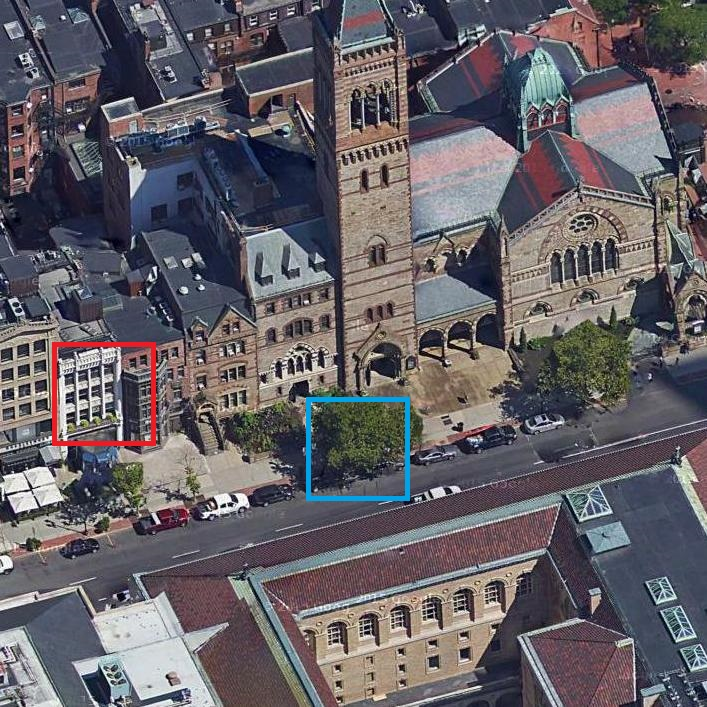
\includegraphics[width=0.23\textwidth]{img/satellite}
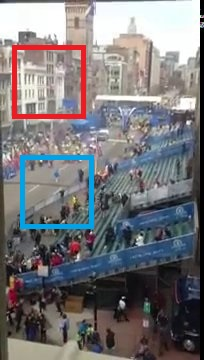
\includegraphics[width=0.13\textwidth]{img/video}
\\[0.1cm]
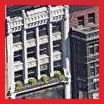
\includegraphics[width=0.10\textwidth]{img/finish_1}
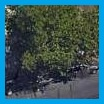
\includegraphics[width=0.10\textwidth]{img/finish_2}
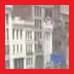
\includegraphics[width=0.10\textwidth]{img/finish_3}
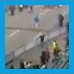
\includegraphics[width=0.10\textwidth]{img/finish_4}
\caption{Comparison between the satellite image (regular appearance) and  the video appearance of the place near Boston Public Library (the finish line of Boston Marathon 2013). The regions in red frames are salient, while those in blue frames are non-salient.}
\label{fig:library}
\end{figure}

% problem formulation and its benefits
The major challenge of event video localization lies in cross-domain large appearance change. 
We observe that despite the large appearance change of the whole environment during the event, certain parts of the environment preserves their daily environment appearance. 
That is, though the whole appearance of each frame is quite different from daily environment image, some regions in a frame are similar to the regions in the daily environment images. 
Based on this key observation, we formulate the task as a joint saliency estimation and matching problem, which simultaneously outputs the matching score and the matched region as supporting evidence. 
Such problem formulation benefits us in three aspects.

First, by explicitly introducing saliency estimation in the model, we are able to distinguish between meaningful matching and meaningless matching. 
For example, the matching between building areas across two images is meaningful since building areas are usually discernible for localization. 
The matching between road and tree areas across two images is meaningless since such matching could occur everywhere and is not helpful to localization. 
Saliency estimation helps to distinguish between these two types of matching and its result will be used to down-weight the meaningless matching and emphasize on meaningful matching in our joint model. 

Second, joint modeling preserves the interdependency between saliency estimation and matching. 
Region saliency is actually domain dependent and depends to matching. 
For example, if a video frame region matches many irrelevant environment images district A , it is not reliable to localize the video in district A based on this frame region. 
That is, this video frame region is not salient in district A. 
Now consider the same video frame region but the environment images of a different district B. 
The same video frame region may only match a few relevant environment images in district B, which means that it is reliable to localize the video based on this frame region in district B. 
That is, the same video frame region turns to be salient in district B. 
In our solution, we capture such interdependency between saliency estimation and matching. 

Third, addition output of matched region makes the system output more explainable. 
For example, when the system fails, the ``matched'' region will be shown to users that there is not enough discernible environment clues in the video content so that it fails reasonably. 
Given such supporting evidence, the users will be more likely to trust the system as they learn to know the capability limit of the system in their usage. 

Our solution is composed of three components: 
\begin{itemize}
\item \emph{Automatic weak label generation: } 
we first generate the labels, which indicate whether two images are matched, by their GPS coordinate. If their distance in the GPS coordinate system is less than a threshold, we label them as matched, otherwise unmatched. 
\item \emph{Saliency estimation with region matching fixed: }
we derive a closed form solution for saliency value, which has an intuitive explanation. 
%Matching based data-driven saliency estimation. We estimate the saliency score of each region based on their matching score to regions in the large-scale database, with a trained model for image matching. 
\item \emph{Self-paced learning for region matching model: }
we leverage self-paced learning to learn region matching model from pseudo labels generated by saliency estimation. 
\end{itemize}

The contributions of this paper are threefold. 
\begin{enumerate}
\item We formulate the event video localization task as a region based joint saliency estimation and matching problem. 
\item We derive an iterative solution to the non-convex optimization problem, which is composed of two steps: closed form solution for saliency estimation and self-paced learning for region matching model. 
\item Our solution output is not only accurate but also interpretable by human beings. 
\end{enumerate}

% section arrangement
The rest of the paper is organized as follows. 
Section~\ref{sec:related} introduces related work. 
Section~\ref{sec:problem} formalizes the problem for the video event localization task. 
Section~\ref{sec:solution} gives the solution to the problem. 
Section~\ref{sec:expr} presents the experiment results. 
Section~\ref{sec:conclusion} draws some conclusions and the work in the future.
